\documentclass[tikz,border=5pt]{standalone}
\usetikzlibrary{arrows.meta,positioning,calc,backgrounds,fit}

\definecolor{ink}{HTML}{243447}
\definecolor{source}{HTML}{E8F1F8}
\definecolor{latent}{HTML}{E4F3EE}
\definecolor{objective}{HTML}{F7EBD0}
\definecolor{evaluation}{HTML}{EFEAF7}
\definecolor{target}{HTML}{F8E7E7}

\begin{document}
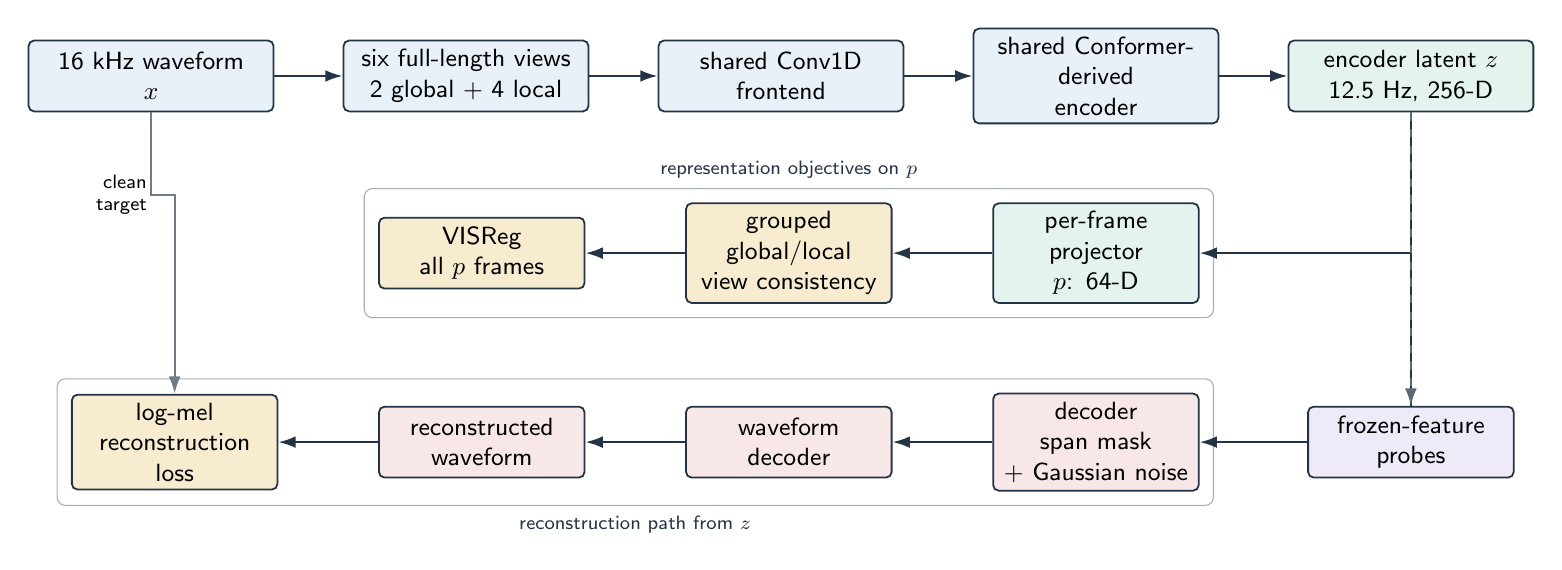
\begin{tikzpicture}[
  font=\sffamily\small,
  box/.style={draw=ink, line width=.65pt, rounded corners=2pt,
    minimum height=9mm, text width=29mm, align=center, inner sep=3pt},
  smallbox/.style={box, text width=24mm},
  flow/.style={-{Latex[length=2.2mm,width=1.5mm]}, draw=ink, line width=.8pt},
  evalflow/.style={flow, dashed, draw=ink!75},
  group/.style={draw=ink!40, rounded corners=3pt, inner sep=5pt}
]
  \node[box, fill=source] (wave) at (0,0) {16 kHz waveform\\$x$};
  \node[box, fill=source] (views) at (4.0,0) {six full-length views\\2 global + 4 local};
  \node[box, fill=source] (front) at (8.0,0) {shared Conv1D\\frontend};
  \node[box, fill=source] (enc) at (12.0,0) {shared Conformer-derived\\encoder};
  \node[box, fill=latent] (z) at (16.0,0) {encoder latent $z$\\12.5 Hz, 256-D};

  \draw[flow] (wave) -- (views);
  \draw[flow] (views) -- (front);
  \draw[flow] (front) -- (enc);
  \draw[flow] (enc) -- (z);

  \node[smallbox, fill=latent] (proj) at (12.0,-2.25) {per-frame projector\\$p$: 64-D};
  \node[smallbox, fill=objective] (cons) at (8.1,-2.25) {grouped global/local\\view consistency};
  \node[smallbox, fill=objective] (vis) at (4.2,-2.25) {VISReg\\all $p$ frames};
  \draw[flow] (z.south) |- (proj.east);
  \draw[flow] (proj) -- (cons);
  \draw[flow] (cons) -- (vis);

  \node[smallbox, fill=target] (corrupt) at (12.0,-4.65) {decoder span mask\\+ Gaussian noise};
  \node[smallbox, fill=target] (decoder) at (8.1,-4.65) {waveform decoder};
  \node[smallbox, fill=target] (recon) at (4.2,-4.65) {reconstructed\\waveform};
  \node[smallbox, fill=objective] (mel) at (0.3,-4.65) {log-mel\\reconstruction loss};
  \draw[flow] (z.south) |- (corrupt.east);
  \draw[flow] (corrupt) -- (decoder);
  \draw[flow] (decoder) -- (recon);
  \draw[flow] (recon) -- (mel);
  \draw[flow, draw=ink!65] (wave.south) -- ++(0,-1.05) -| node[pos=.13,left,font=\sffamily\scriptsize,align=right] {clean\\target} (mel.north);

  \node[smallbox, fill=evaluation] (probes) at (16.0,-4.65) {frozen-feature\\probes};
  \draw[evalflow] (z) -- (probes);

  \begin{scope}[on background layer]
    \node[group, fit=(proj)(cons)(vis), label={[font=\sffamily\scriptsize,ink]above:representation objectives on $p$}] {};
    \node[group, fit=(corrupt)(decoder)(recon)(mel), label={[font=\sffamily\scriptsize,ink]below:reconstruction path from $z$}] {};
  \end{scope}
\end{tikzpicture}
\end{document}
